\chapter[Desenvolvimento dos modelos de treinamento]{Desenvolvimento dos modelos de treinamento}
\addcontentsline{toc}{chapter}{Desenvolvimento dos modelos de treinamento}
\label{chap:desenvolvimento}

O problema central que o modelo de aprendizado federado busca resolver reside na exposição potencial de dados sensíveis quando centralizados em um único servidor para treinamento de modelos de IA. Em vez de enviar os dados dos dispositivos para um servidor central, onde poderiam ser acessados ou comprometidos, o aprendizado federado propõe um paradigma descentralizado no qual os dispositivos realizam o treinamento localmente, compartilhando apenas os parâmetros do modelo (como pesos e gradientes) com o servidor central. Esta abordagem permite que os dispositivos colaborem no desenvolvimento de um modelo global sem nunca expor os dados locais. 

A estruturação do problema foi conduzida considerando-se um cenário prático, onde múltiplos dispositivos, cada um contendo dados não identicamente distribuídos (não-IID), contribuem para o treinamento de um modelo de classificação de imagens (utilizando o conjunto de dados MNIST como referência). Este cenário foi escolhido por refletir uma situação comum em aplicações reais, onde dados como registros de saúde, preferências de usuários ou informações financeiras são distribuídos entre dispositivos pessoais e não podem ser compartilhados diretamente por questões de privacidade e conformidade com regulamentos como o GDPR. Assim, a metodologia abrange a implementação de um modelo federado que deve ser capaz de aprender de maneira eficiente e precisa a partir de dados dispersos, preservando a privacidade, e enfrenta desafios como a heterogeneidade dos dispositivos, a variabilidade da conectividade de rede e a necessidade de garantir a convergência do modelo global. A escolha do aprendizado federado, mais especificamente do processo Federated Averaging (FedAvg), é justificada pela sua capacidade de operar eficientemente em ambientes com essas características, buscando balancear a necessidade de proteção dos dados com a performance do modelo treinado.

\section{Implementação do Modelo de Aprendizado Federado}

Para melhor entendimento, foi dividido em seções a implementação do código do modelo de aprendizado federado. Cada seção abordará uma etapa do desenvolvimento do modelo e por fim será apresentado o código completo.

\subsection{Definição do Modelo Keras}

\begin{figure}[ht]
    \centering
    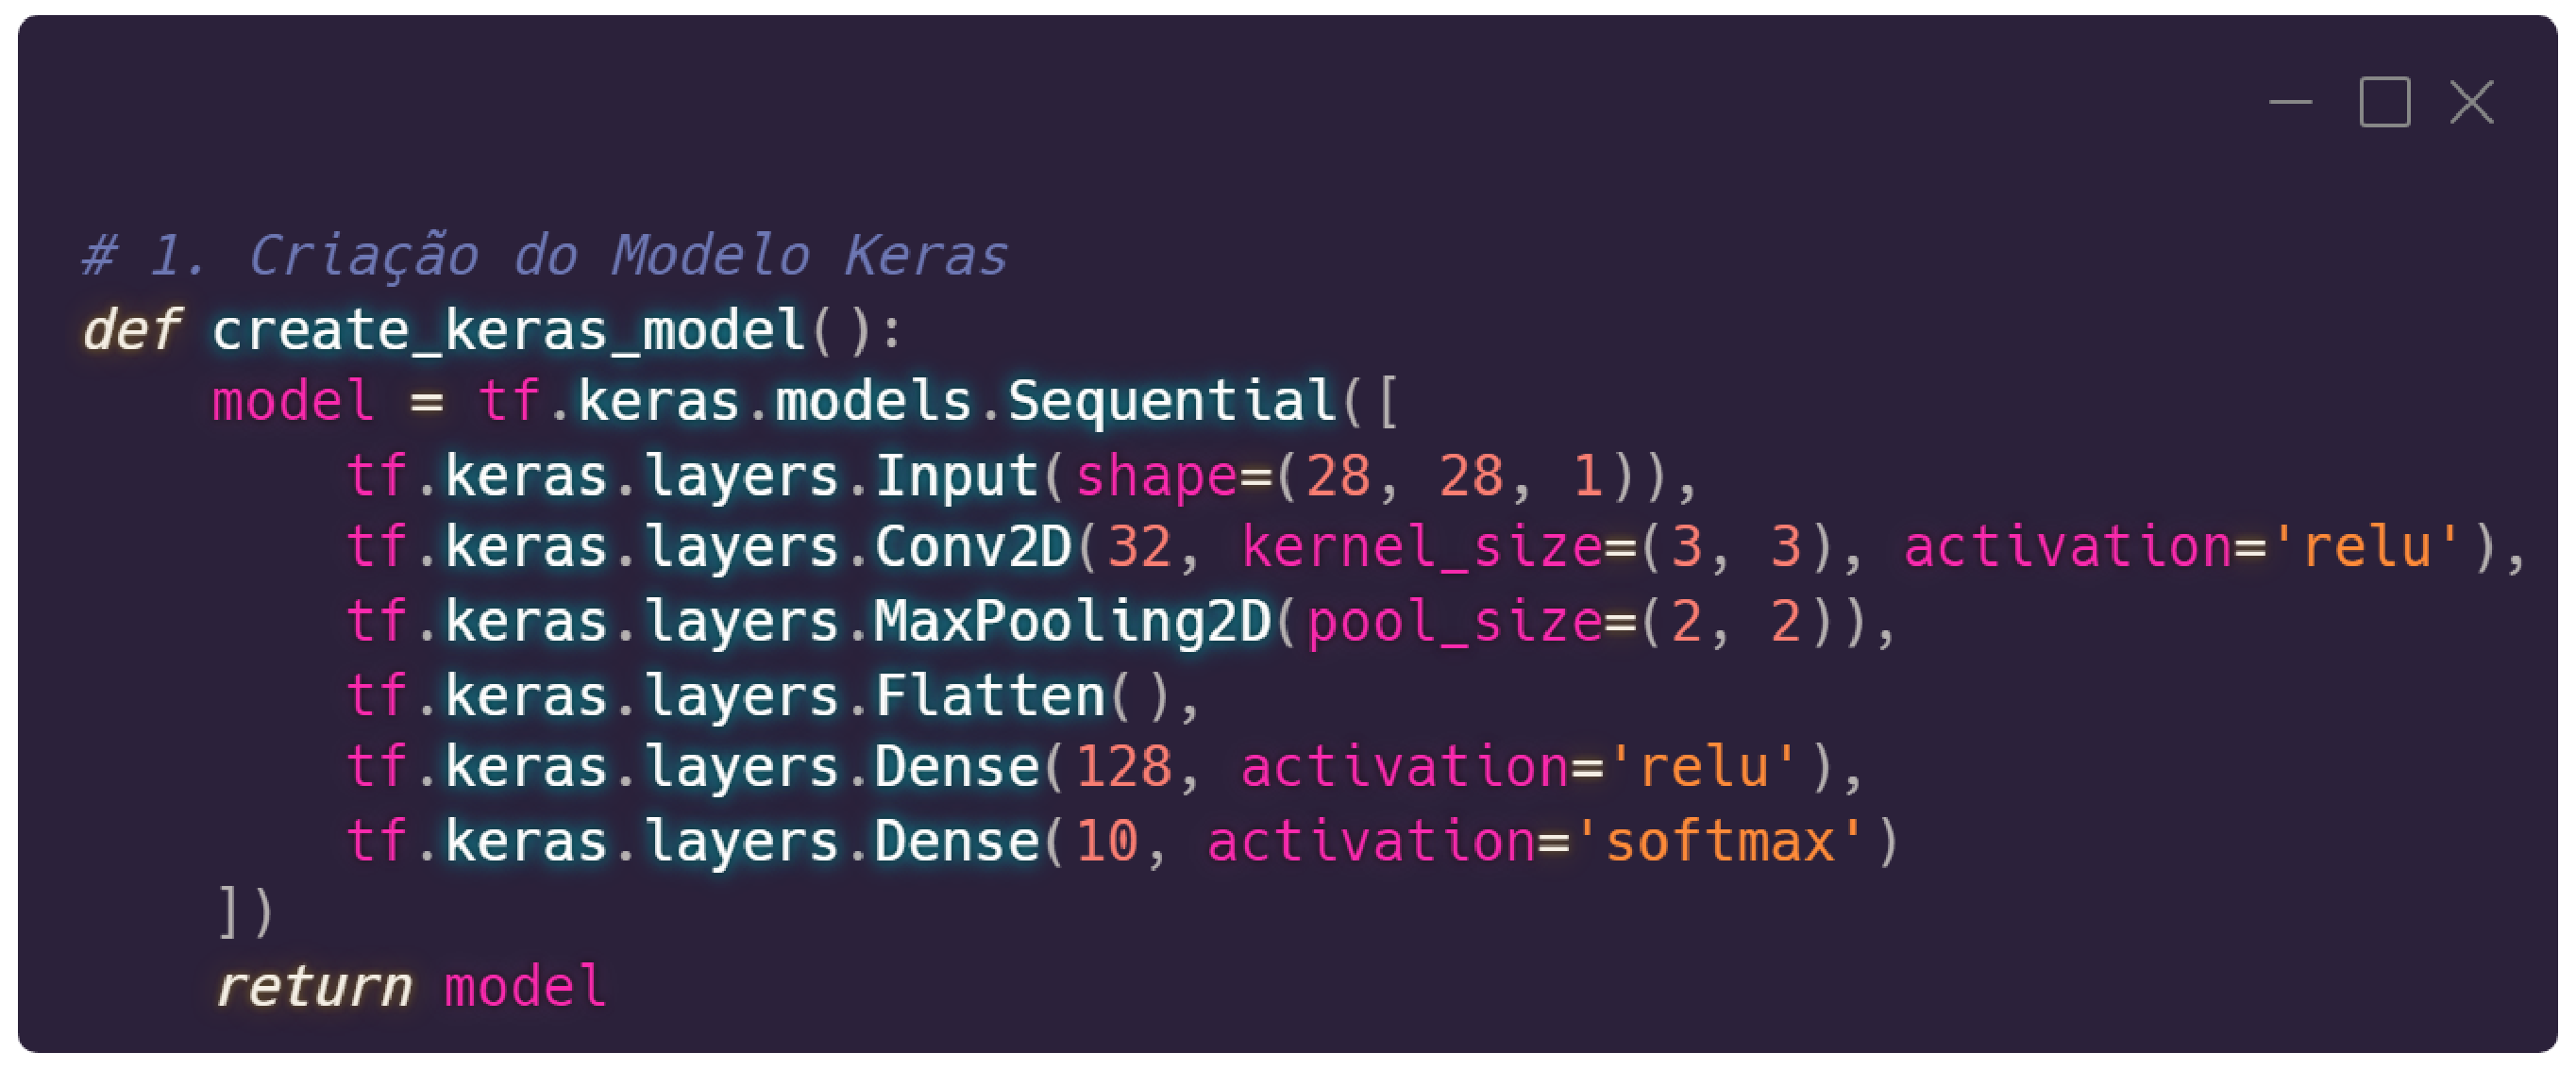
\includegraphics[scale=0.25]{figuras/kerasModel.eps}
    \caption{Criação do Modelo Keras.}
    \label{fig:kerasModel}
\end{figure}

A criação do modelo Keras neste ponto é feita utilizando uma rede neural convolucional (CNN) simples, apropriada para a tarefa de classificação de imagens. A escolha de uma CNN com camadas convolucionais (Conv2D) é natural para lidar com o conjunto de dados MNIST, que consiste em imagens de dígitos manuscritos de 28x28 pixels em escala de cinza. A arquitetura definida é clássica: começa com uma camada convolucional para extrair características visuais seguidas de uma camada de pooling (MaxPooling2D) para reduzir dimensionalidade e complexidade, além de prevenir overfitting. A camada Flatten é utilizada para achatar a saída da camada convolucional para um formato unidimensional, o que permite a conexão com a camada densa (Dense), que atua como classificador. A escolha da função de ativação ReLU nas camadas intermediárias é estratégica, pois introduz não-linearidade, tornando a rede capaz de aprender relações complexas nos dados. A camada final usa softmax, adequada para tarefas de classificação multiclasse, já que o MNIST contém 10 classes (dígitos de 0 a 9). Essa arquitetura é uma escolha padrão para começar com a classificação de imagens simples e fornece uma base sólida para implementar um modelo federado.

\subsection{Construção do Modelo Federado}

\begin{figure}[ht]
    \centering
    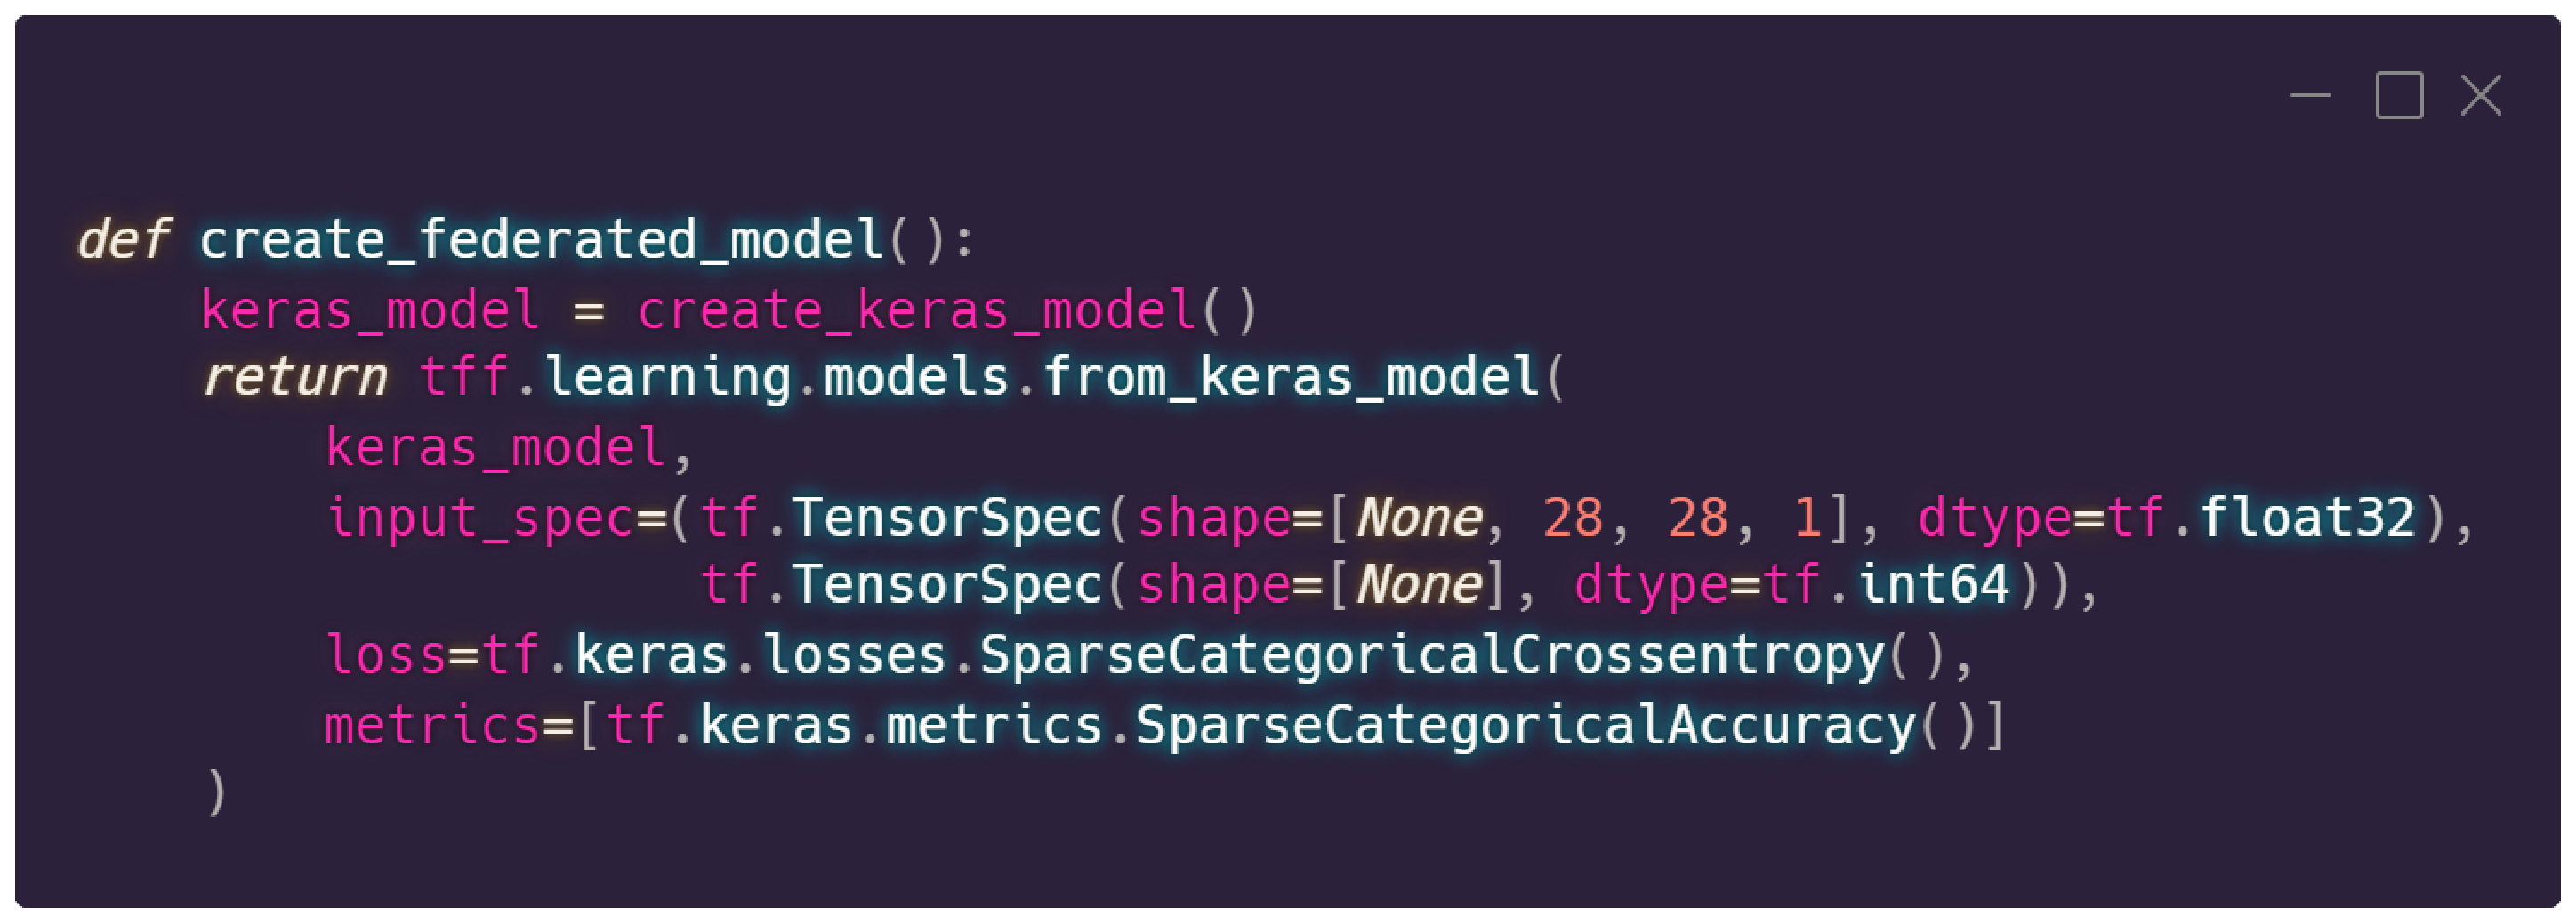
\includegraphics[scale=0.25]{figuras/federatedModel.eps}
    \caption{Construção do modelo federado.}
    \label{fig:federatedModel}
\end{figure}

O modelo federado é construído a partir do modelo Keras criado anteriormente, mas com algumas adaptações específicas para o contexto federado. A função \texttt{tff.learning.models.from\_keras\_model} é usada para integrar o modelo Keras ao fluxo de aprendizado federado no TensorFlow Federated. A especificação de entrada (\textit{input\_spec}) define como os dados serão representados em termos de tipo e forma, essencial para garantir que o modelo possa lidar corretamente com o formato dos dados federados, onde múltiplos dispositivos podem ter seus próprios subconjuntos de dados. A função de perda escolhida é a \textit{SparseCategoricalCrossentropy}, ideal para tarefas de classificação onde os rótulos das classes são inteiros. A métrica \textit{SparseCategoricalAccuracy} foi selecionada por ser apropriada para medir a precisão em tarefas de classificação de rótulos discretos. Essa escolha mantém consistência com as práticas padrão para modelos de classificação e permite uma transição tranquila para um ambiente federado.

\subsection{Construção do Processo de Federado}

\begin{figure}[ht]
    \centering
    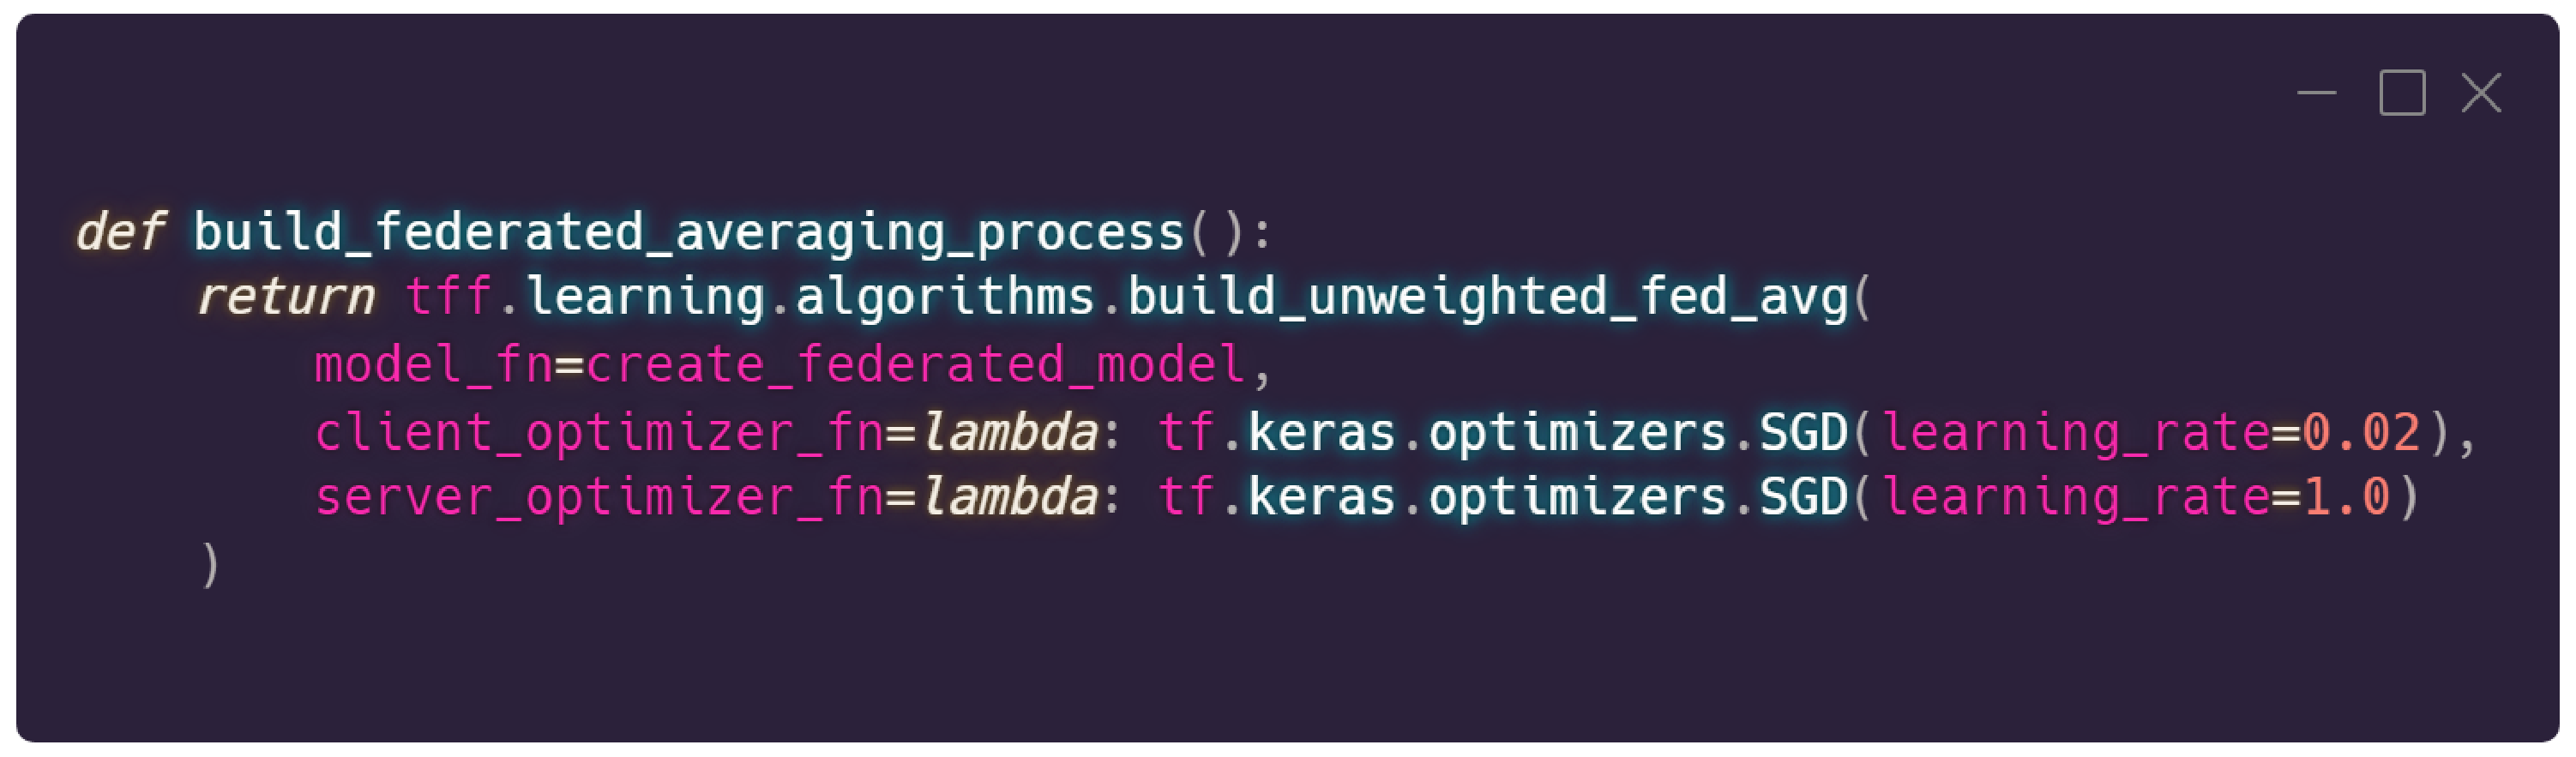
\includegraphics[scale=0.25]{figuras/federatedProccess.eps}
    \caption{Construção do Processo de Federado.}
    \label{fig:federatedProccess}
\end{figure}

A escolha do algoritmo de treinamento federado, o \textit{FedAvg} (Federated Averaging), é uma das mais utilizadas em aprendizado federado por ser simples e eficaz. O \textit{FedAvg} permite que cada cliente (dispositivo) atualize localmente o modelo com base em seus dados privados, e depois envia essas atualizações para o servidor, onde elas são agregadas. A função \texttt{build\_unweighted\_fed\_avg} constrói esse processo de agregação sem ponderar a contribuição de cada cliente, o que é adequado para cenários com uma distribuição de dados homogênea entre os clientes. 

Para a otimização, foi escolhido o \textit{SGD} (Stochastic Gradient Descent) tanto para os clientes quanto para o servidor, um otimizador padrão em redes neurais, por sua simplicidade e eficiência em problemas de classificação. A taxa de aprendizado para os clientes foi ajustada para um valor menor (0.02) para garantir que cada cliente faça pequenas atualizações locais, evitando grandes variações que poderiam desestabilizar o treinamento. Para o servidor, a taxa de aprendizado foi configurada para um valor mais alto (1.0), uma escolha comum para permitir que a média das atualizações dos clientes seja aplicada de forma mais agressiva no modelo global.

\subsection{Preparação dos Dados}

\begin{figure}[ht]
    \centering
    \includegraphics[scale=0.2]{figuras/dataPreparation.eps}
    \caption{Preparação dos dados.}
    \label{fig:dataPreparation}
\end{figure}

A preparação dos dados é uma etapa fundamental, especialmente em aprendizado federado, onde os dados são distribuídos entre diferentes ``clientes'' (dispositivos). O processo de preparação transforma as imagens do MNIST para o formato adequado, normalizando os dados para a faixa de valores [0, 1], o que facilita o treinamento, já que o modelo tende a convergir melhor com dados normalizados. A função \texttt{preprocess} garante que cada lote de dados seja preparado corretamente, convertendo o formato para tensores e realizando o \textit{batching} (agrupamento em lotes) de 20 amostras. A escolha de repetir os dados (\texttt{repeat(10)}) aumenta o número de amostras disponíveis para treinamento em cada cliente. 

A função \texttt{create\_client\_data} é responsável por distribuir os dados de maneira federada entre os clientes simulados, dividindo igualmente o conjunto de dados entre 10 clientes. Essa abordagem permite que cada cliente tenha uma quantidade razoável de dados, simulando cenários do mundo real, onde os dispositivos (como smartphones) possuem seus próprios subconjuntos de dados.

\subsection{Treinamento do Modelo Federado}

\begin{figure}[ht]
    \centering
    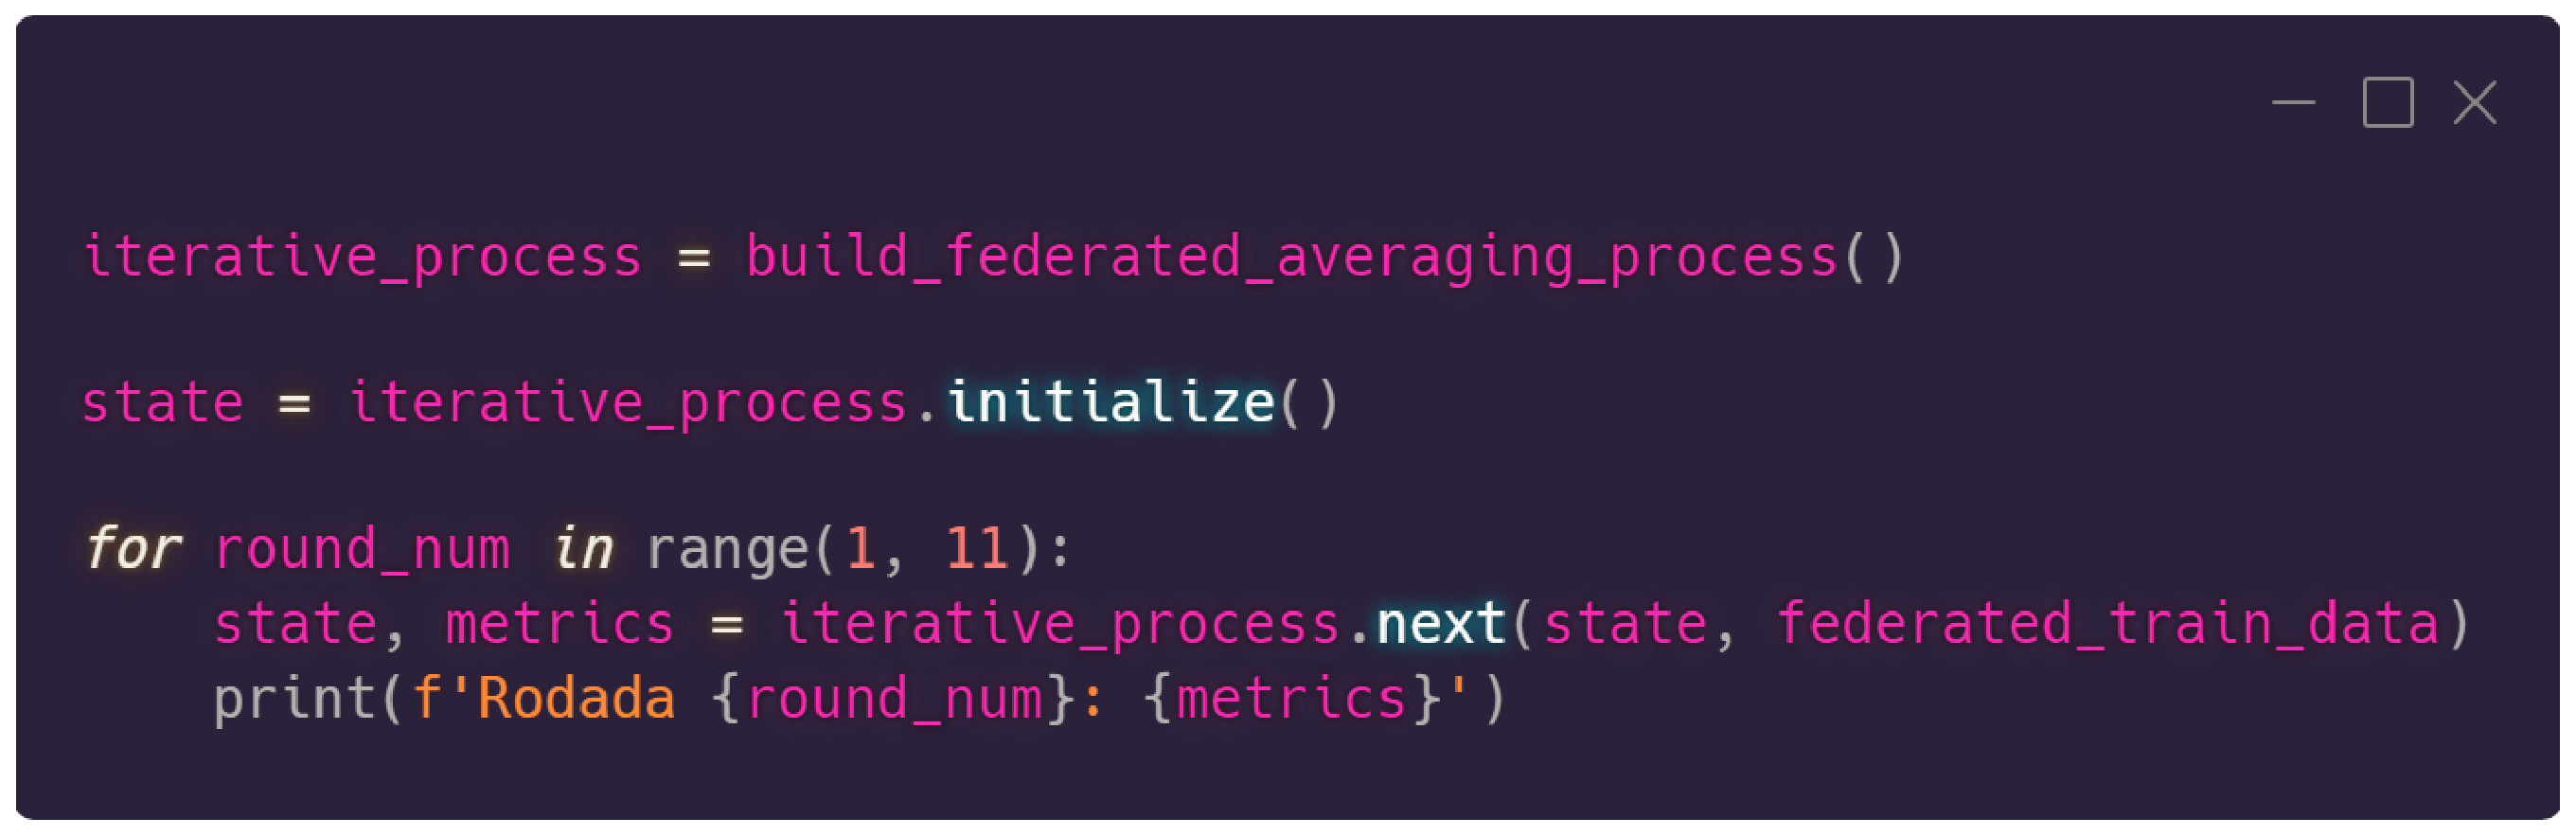
\includegraphics[scale=0.25]{figuras/modelTraining.eps}
    \caption{Treinamento do modelo federado.}
    \label{fig:modelTraining}
\end{figure}

O treinamento é executado através de um processo iterativo, onde o modelo é treinado em múltiplas rodadas. A escolha de 10 rodadas de treinamento permite uma observação inicial do comportamento do modelo federado sem sobrecarregar o sistema. Em cada rodada, os clientes locais treinam o modelo com seus dados privados e enviam as atualizações para o servidor central, onde as atualizações são agregadas para formar um modelo global atualizado. O uso da função \texttt{next} no TensorFlow Federated aplica a agregação de \textit{FedAvg}, onde as médias das atualizações dos clientes são calculadas. O feedback das métricas de cada rodada permite acompanhar a evolução do modelo, especialmente em termos de precisão (via \textit{SparseCategoricalAccuracy}), oferecendo uma visão clara de como o modelo está se ajustando aos dados federados ao longo do tempo.

\section{Implementação do Modelo de Aprendizado Centralizado}

Para criar um modelo de treinamento centralizado, foi realizado um processo semelhante ao do aprendizado federado utilizando a mesma biblioteca de dados (MNIST) e as mesmas ferramentas, apenas sem a distribuição de dados entre dispositivos. Esse modelo será utilizado para comparação com o modelo federado desenvolvido anteriormente, possibilitando a avaliação do impacto do aprendizado centralizado versus o aprendizado federado na preservação da privacidade e desempenho.

\subsection{Criação do Modelo de Aprendizado Centralizado}

\subsubsection{Definição do Modelo Keras}

\begin{figure}[ht]
    \centering
    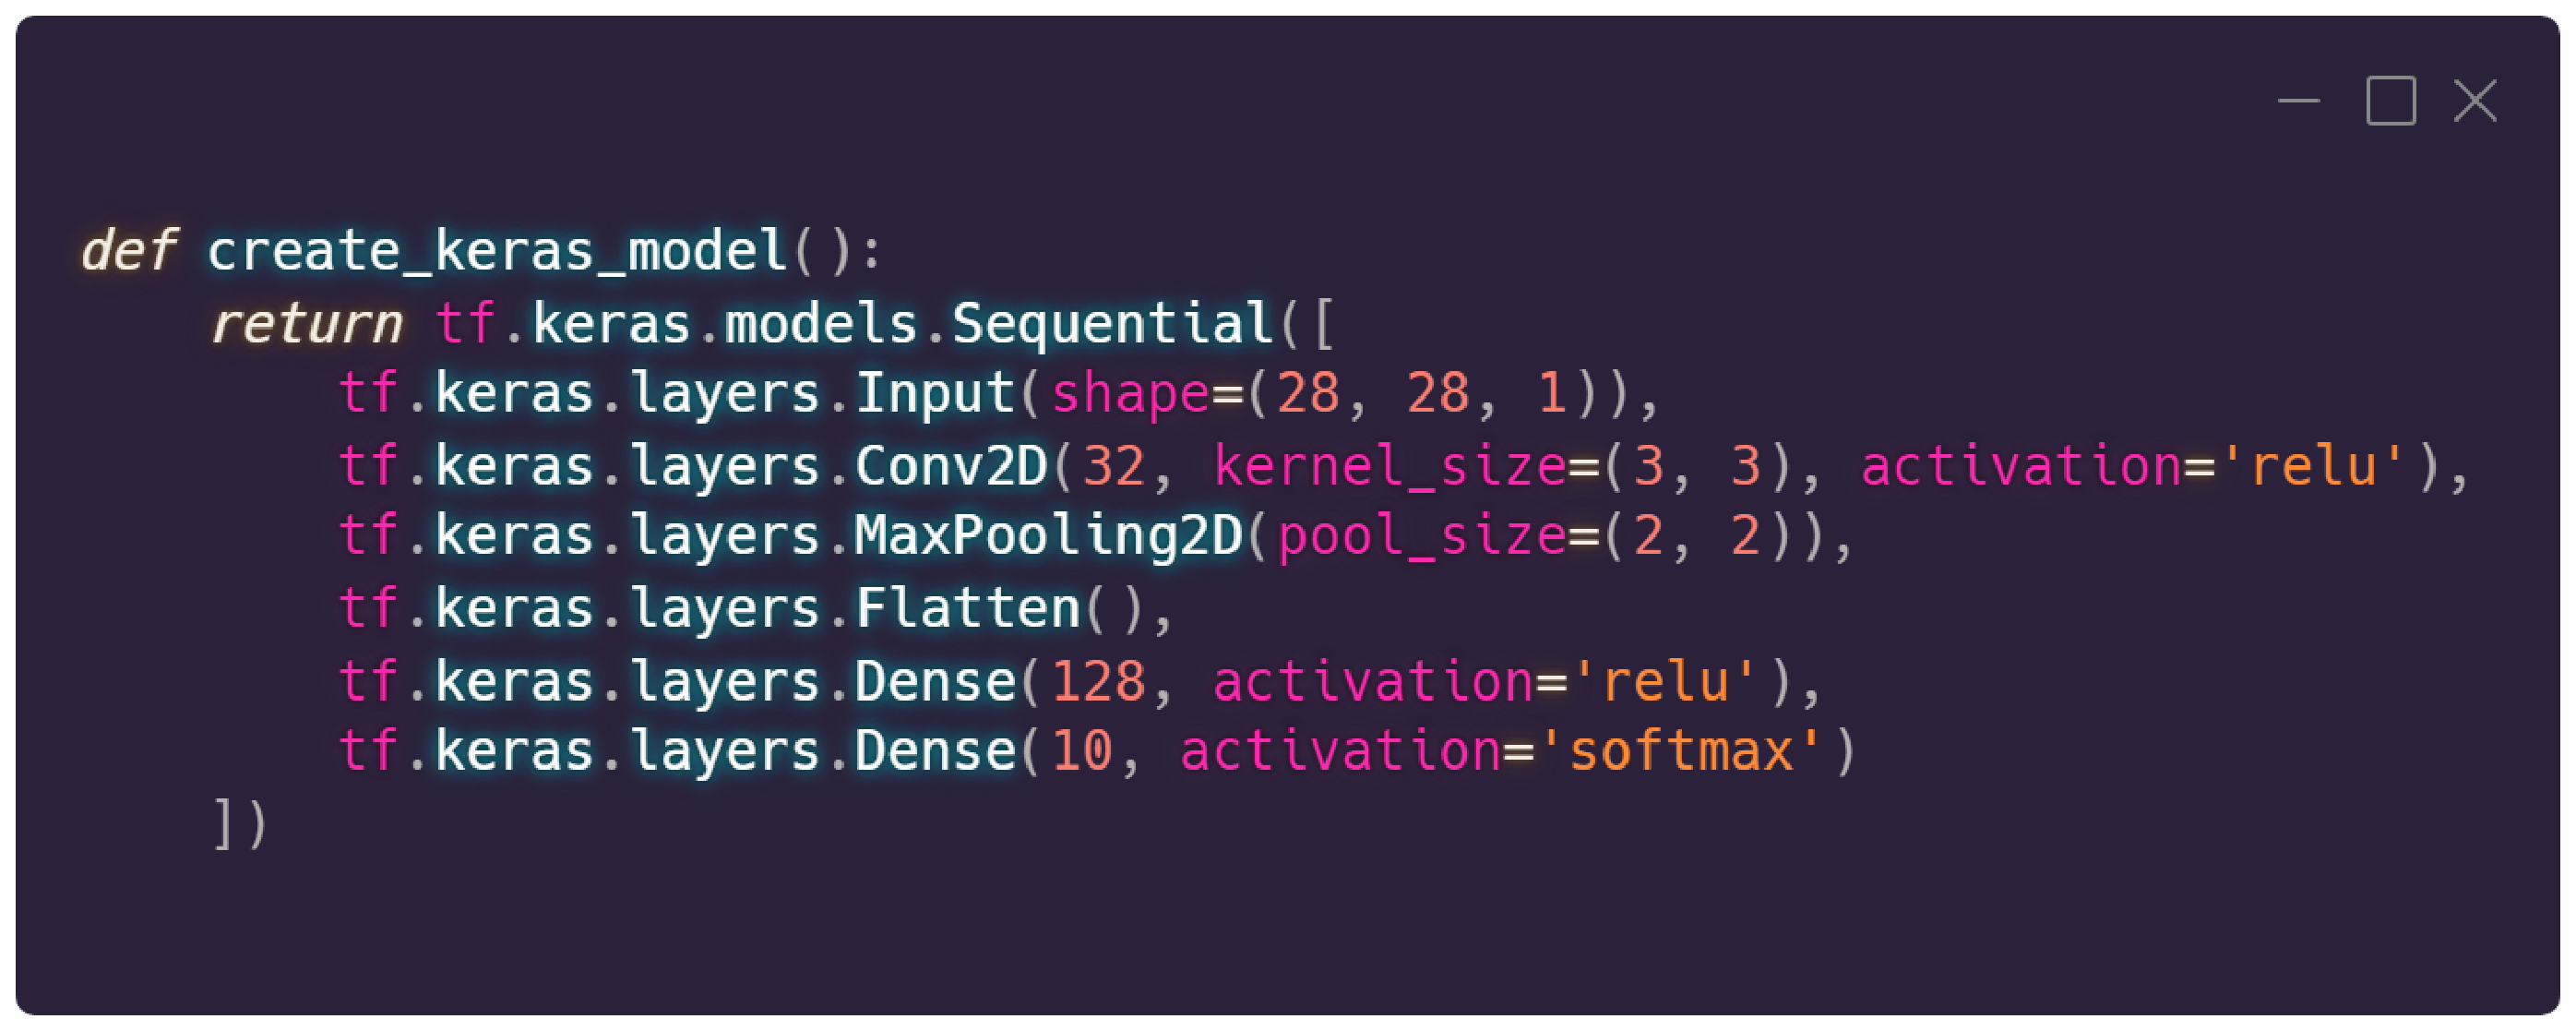
\includegraphics[scale=0.25]{figuras/kerasCentralized.eps}
    \caption{Definição do Modelo Keras.}
    \label{fig:kerasCentralized}
\end{figure}

Comparando com o modelo federado, a estrutura básica do modelo é a mesma, mas no federado, a criação do modelo é encapsulada em uma função TFF para suportar o treinamento distribuído, e o modelo não é compilado no momento da criação. O modelo centralizado é mais direto e é compilado imediatamente, o que simplifica a implementação.

\subsubsection{Carregamento e Preparação dos Dados}

\begin{figure}[ht]
    \centering
    \includegraphics[scale=0.25]{figuras/dataPrepCentralized.eps}
    \caption{Carregamento e Preparação dos Dados.}
    \label{fig:dataPrepCentralized}
\end{figure}

Comparado ao modelo federado, o modelo centralizado lida com dados de forma mais direta e monolítica. No modelo federado, os dados são distribuídos entre os clientes e processados em batches menores para simular um cenário de aprendizado distribuído.

\subsubsection{Criação e Compilação do Modelo Centralizado}

\begin{figure}[ht]
    \centering
    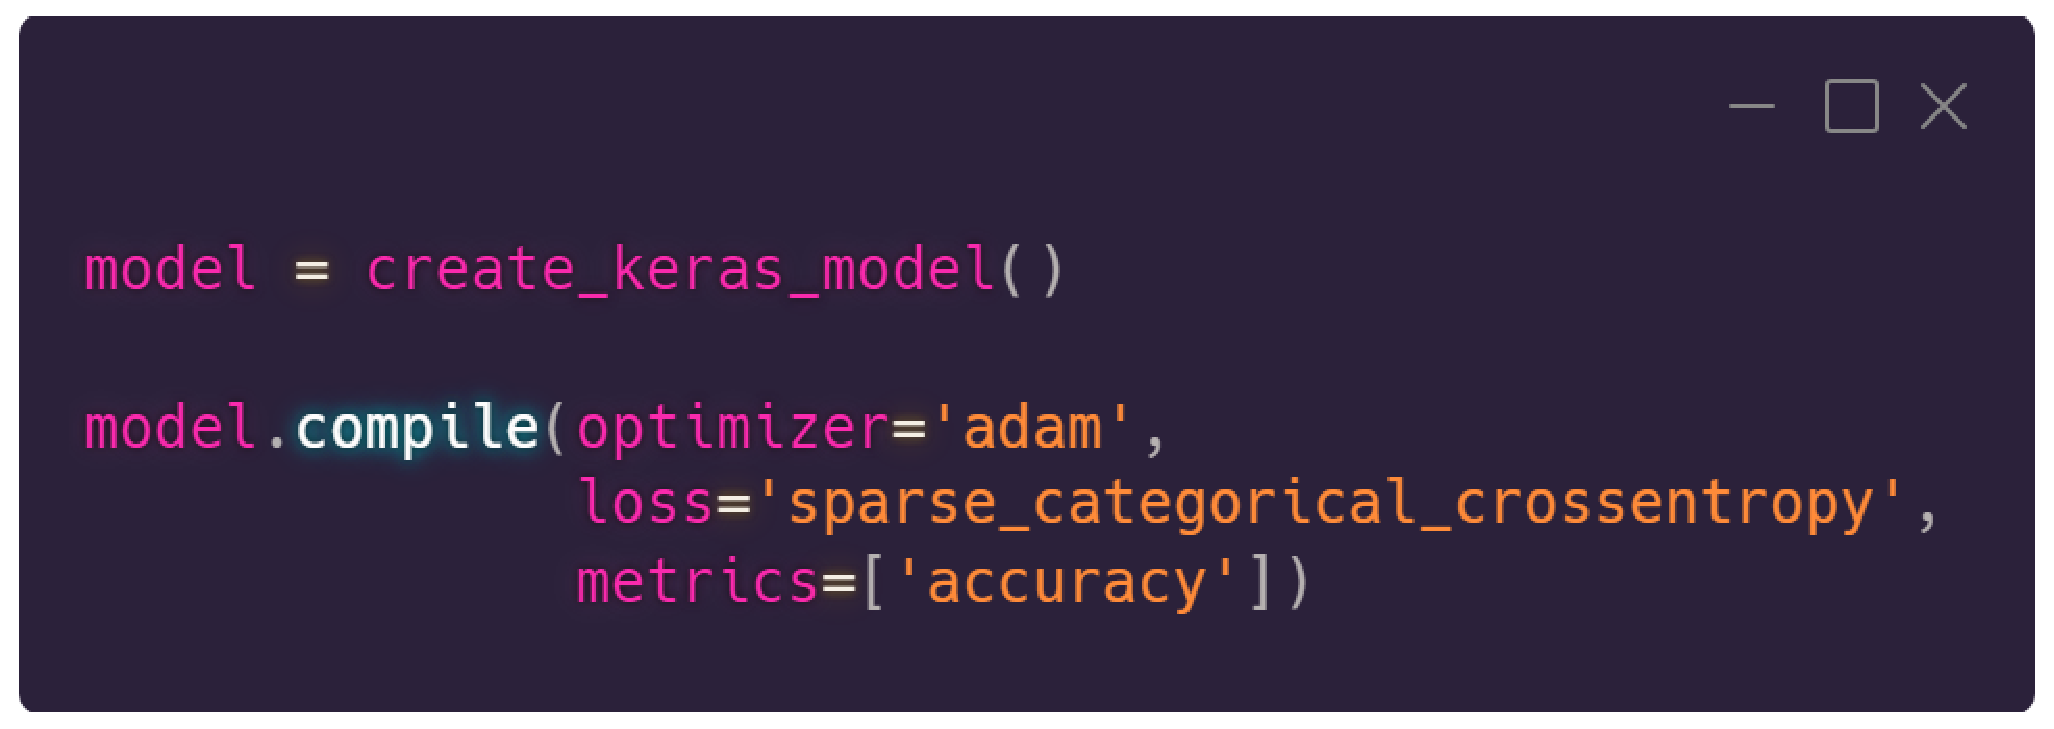
\includegraphics[scale=0.25]{figuras/compileModelCentralized.eps}
    \caption{Criação e Compilação do Modelo Centralizado.}
    \label{fig:compileModelCentralized}
\end{figure}

No modelo federado, a compilação não ocorre na função de criação do modelo. Em vez disso, é feita na configuração do processo de treinamento, onde funções de perda e métricas são especificadas no contexto federado.

\subsubsection{Treinamento do Modelo Centralizado}

\begin{figure}[ht]
    \centering
    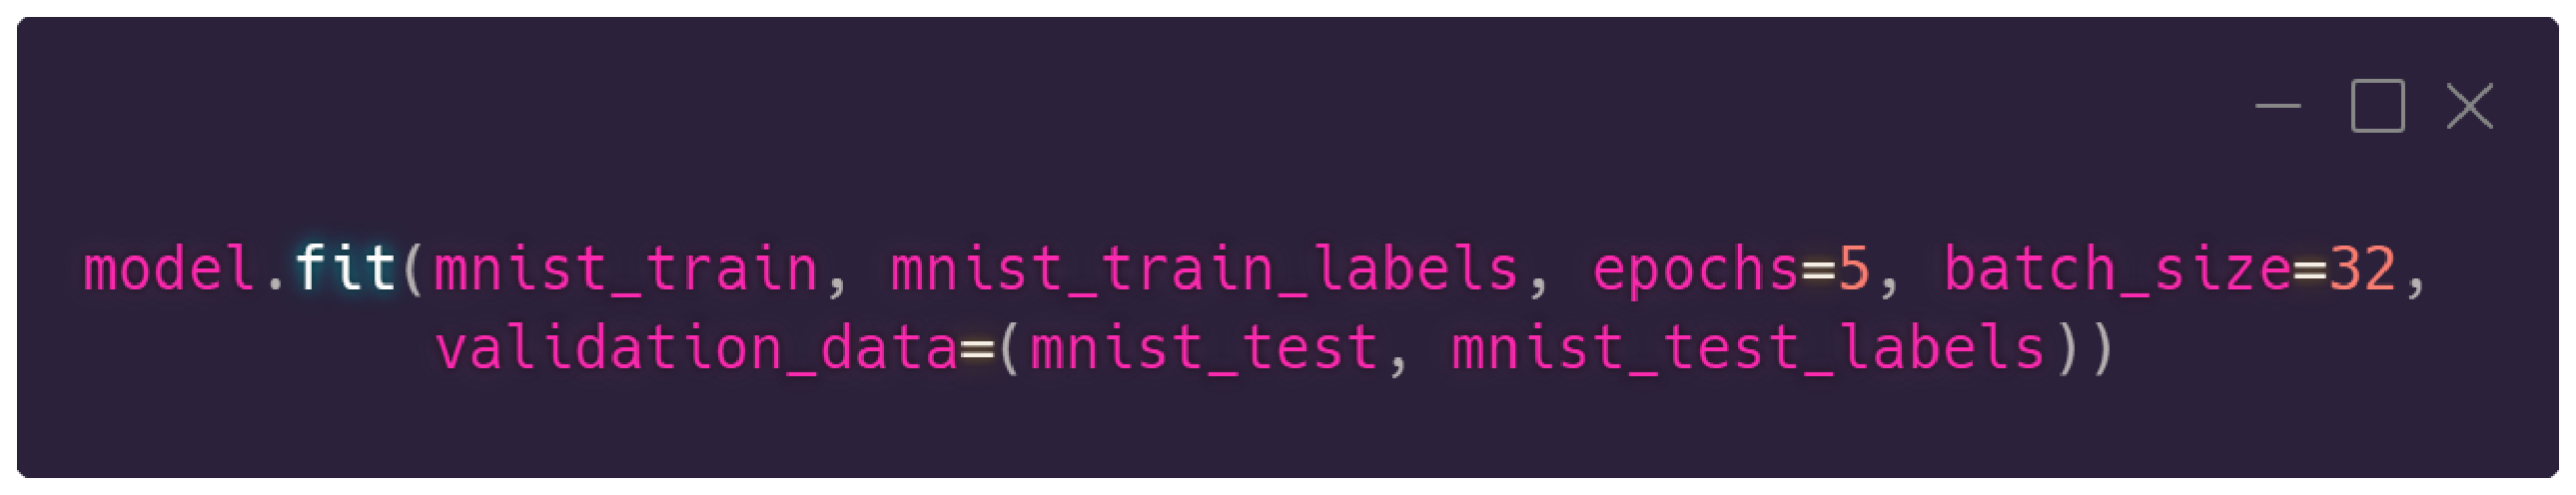
\includegraphics[scale=0.25]{figuras/trainingCentralized.eps}
    \caption{Treinamento do modelo Centralizado.}
    \label{fig:trainingCentralized}
\end{figure}

No modelo federado, o treinamento é distribuído entre vários clientes e o processo de treinamento é coordenado centralmente. A atualização dos pesos é feita de maneira agregada, o que é uma abordagem fundamentalmente diferente da atualização direta utilizada no treinamento centralizado.

\subsubsection{Avaliação do Modelo}

\begin{figure}[ht]
    \centering
    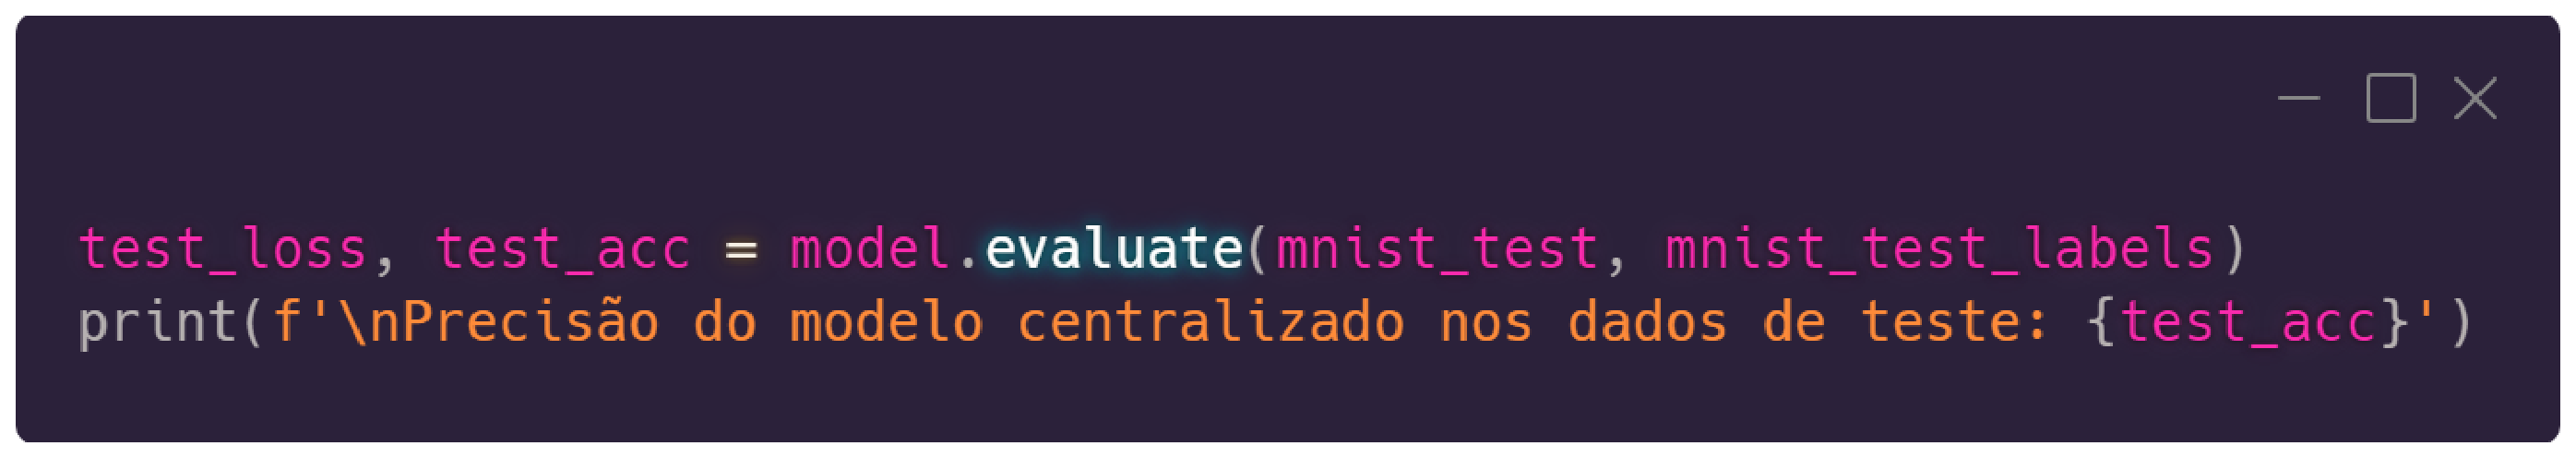
\includegraphics[scale=0.25]{figuras/testCentralized.eps}
    \caption{Avaliação do Modelo.}
    \label{fig:testCentralized}
\end{figure}

A avaliação do modelo é feita usando \texttt{model.evaluate()}, que calcula a perda e a precisão do modelo nos dados de teste. Isso fornece uma medida direta do desempenho do modelo em dados que não foram usados durante o treinamento, ajudando a verificar sua capacidade de generalização. No contexto do aprendizado federado, a avaliação é geralmente realizada de forma agregada após o treinamento federado ter sido concluído. A abordagem é diferente, pois a avaliação pode ser feita em vários conjuntos de dados de clientes para refletir a performance geral do modelo distribuído.

\section{Justificativa}

A escolha do processo de \textbf{Federated Averaging (FedAvg)} foi baseada em sua eficácia e simplicidade para a implementação de aprendizado federado em cenários onde a privacidade dos dados é uma preocupação central. A seguir, discutiremos as razões específicas para a escolha do FedAvg, suas vantagens e desvantagens, e os modelos de treinamento tradicionais que poderiam ser utilizados para comparar a performance.

\subsection{Razões para a Escolha do FedAvg}

O \textbf{FedAvg} é amplamente reconhecido e utilizado como uma das abordagens mais eficientes para o aprendizado federado, especialmente em contextos onde os dados são distribuídos entre vários clientes (dispositivos) que possuem capacidade computacional limitada. Ele opera através da média ponderada dos pesos dos modelos treinados localmente em cada cliente. Algumas das principais razões para a escolha do FedAvg incluem:

1. Simplicidade de Implementação: O FedAvg é relativamente fácil de implementar, tanto em termos de código quanto em infraestrutura. Ele não requer modificações complexas no modelo original e é compatível com a maioria dos modelos de aprendizado de máquina.

2. Eficiência em Ambientes Heterogêneos: Em cenários onde os clientes possuem capacidades computacionais variadas e dados não IID (independentemente e identicamente distribuídos), o FedAvg tem se mostrado robusto e eficaz. Ele permite que cada cliente contribua de acordo com sua capacidade, o que é ideal para dispositivos com diferentes níveis de poder computacional e conectividade.

3. Privacidade Preservada: Como o FedAvg realiza o treinamento localmente nos dispositivos dos clientes e apenas os pesos dos modelos (não os dados) são enviados para o servidor central, ele ajuda a preservar a privacidade dos dados.

\subsection{Vantagens do FedAvg}

1. Escalabilidade: FedAvg é altamente escalável, sendo capaz de lidar com milhares de dispositivos clientes. A abordagem distribuída minimiza a necessidade de centralização de dados, reduzindo os gargalos associados ao processamento em larga escala.

2. Flexibilidade: FedAvg pode ser aplicado a uma ampla variedade de modelos de aprendizado de máquina, desde redes neurais profundas até modelos mais simples, tornando-o versátil em diferentes cenários de aplicação.

3. Resiliência a Dados Não IID: Em muitos cenários do mundo real, os dados disponíveis em diferentes dispositivos não seguem uma distribuição IID. O FedAvg consegue lidar razoavelmente bem com essas discrepâncias.

\subsection{Desvantagens do FedAvg}

1. Convergência Mais Lenta: Devido à natureza distribuída e à variabilidade entre os dispositivos, a convergência do FedAvg pode ser mais lenta comparada a métodos centralizados, especialmente em casos onde os dados são altamente desbalanceados entre os clientes.

2. Dependência de Conectividade: O FedAvg requer que os dispositivos clientes enviem periodicamente seus modelos atualizados ao servidor central. Em ambientes com conectividade de rede instável ou dispositivos com pouca energia, isso pode se tornar um desafio.

3. Sobrecarga Computacional e de Comunicação: Embora o FedAvg minimize a necessidade de centralização de dados, ele ainda requer que os dispositivos locais realizem computações significativas e participem regularmente da comunicação com o servidor, o que pode ser oneroso para dispositivos de baixa potência.

\section{Código e aplicação dos modelos}

Esta seção apresenta o código completo desenvolvido para a implementação do modelo de aprendizado federado utilizando o TensorFlow Federated.

A segunda parte dessa seção apresenta a implementação do modelo de treinamento centralizado que será utilizado para comparação com o modelo federado. O código é estruturado de forma semelhante ao modelo federado, mas com a diferença de que os dados são centralizados em um único servidor para treinamento.

\subsection{Implementação completa do Modelo de Aprendizado Federado}

\begin{figure}[ht]
    \centering
    \includegraphics[scale=0.2]{figuras/CodeFederatedLearning.eps}
    \caption{Implementação do modelo de Aprendizado Federado.}
    \label{fig:CodeFederatedLearning}
\end{figure}

\subsection{Implementação completa do Modelo de Aprendizado Centralizado}

\begin{figure}[ht]
    \centering
    \includegraphics[scale=0.2]{figuras/centralizedModel.eps}
    \caption{Implementação do Modelo de Aprendizado Centralizado.}
    \label{fig:centralizedModel}
\end{figure}